% rasti_template.tex 
%
% LaTeX template for creating an RASTI paper
%
% v1.0 released 12 November 2021
% (version numbers match those of rasti.cls)
%
% Copyright (C) Royal Astronomical Society 2021
% Authors:
% Peter Jones (OUP, adapted from mnras_template.tex, author Keith T. Smith (Royal Astronomical Society))

% Change log
%
% v1.0 November 2021
%    Adapted from mnras_template.tex


%%%%%%%%%%%%%%%%%%%%%%%%%%%%%%%%%%%%%%%%%%%%%%%%%%
% Basic setup. Most papers should leave these options alone.
%\documentclass[fleqn,usenatbib,referee]{rasti}
\documentclass[fleqn,usenatbib]{rasti}

% RASTI is set in Times font. If you don't have this installed (most LaTeX
% installations will be fine) or prefer the old Computer Modern fonts, comment
% out the following line
\usepackage{newtxtext,newtxmath}
% Depending on your LaTeX fonts installation, you might get better results with one of these:
%\usepackage{mathptmx}
%\usepackage{txfonts}

% Use vector fonts, so it zooms properly in on-screen viewing software
% Don't change these lines unless you know what you are doing
\usepackage[T1]{fontenc}

% Allow "Thomas van Noord" and "Simon de Laguarde" and alike to be sorted by "N" and "L" etc. in the bibliography.
% Write the name in the bibliography as "\VAN{Noord}{Van}{van} Noord, Thomas"
\DeclareRobustCommand{\VAN}[3]{#2}
\let\VANthebibliography\thebibliography
\def\thebibliography{\DeclareRobustCommand{\VAN}[3]{##3}\VANthebibliography}


%%%%% AUTHORS - PLACE YOUR OWN PACKAGES HERE %%%%%

% Only include extra packages if you really need them. Common packages are:
\usepackage{graphicx}	% Including figure files
\usepackage{amsmath}	% Advanced maths commands
%% \usepackage{amssymb}	% Extra maths symbols
\usepackage{aas_macros}
\usepackage{svg}
\usepackage{pdflscape}
%%%%%%%%%%%%%%%%%%%%%%%%%%%%%%%%%%%%%%%%%%%%%%%%%%

%%%%% AUTHORS - PLACE YOUR OWN COMMANDS HERE %%%%%

% Please keep new commands to a minimum, and use \newcommand not \def to avoid
% overwriting existing commands. Example:
%\newcommand{\pcm}{\,cm$^{-2}$}	% per cm-squared
\newcommand{\msun}{\mathcal{M}_{\sun}}
\newcommand{\orcid}[1]{\href{https://orcid.org/#1}{\includesvg[width=10pt]{orcid}}}

%%%%%%%%%%%%%%%%%%%%%%%%%%%%%%%%%%%%%%%%%%%%%%%%%%

%%%%%%%%%%%%%%%%%%% TITLE PAGE %%%%%%%%%%%%%%%%%%%

% Title of the paper, and the short title which is used in the headers.
% Keep the title short and informative.
\title[RASCAL]{Ransac Assisted Spectral CALibration (RASCAL) -- Towards automated spectral wavelength calibration}

% The list of authors, and the short list which is used in the headers.
% If you need two or more lines of authors, add an extra line using \newauthor
\author[J. Veitch-Michaelis and M. C. Lam]{
J. Veitch-Michaelis$^{1\,\orcid{0000-0003-2780-7843}}$\thanks{Contact e-mail: \href{mailto:joshualeo.veitchmichaelis@inf.ethz.ch}{joshualeo.veitchmichaelis@inf.ethz.ch}}
M. C. Lam$^{2\,\orcid{0000-0002-9347-2298}}$\\
% List of institutions
$^{1}$Dep. Informatik, STF H 313, Stampfenbachstrasse 114, 8092 Zürich, Switzerland\\
$^{2}$School of Physics and Astronomy, Tel Aviv University, Tel Aviv, Israel 69978\\
}

% These dates will be filled out by the publisher
\date{Accepted XXX. Received YYY; in original form ZZZ}

% Enter the current year, for the copyright statements etc.
\pubyear{2022}

% Don't change these lines
\begin{document}
\label{firstpage}
\pagerange{\pageref{firstpage}--\pageref{lastpage}}
\maketitle

% Abstract of the paper
\begin{abstract}
%%%%%%%%%%%%%%%%%%%%%%%%%%%%%%%%%%%%%%%%%%%%%%%%%%%%%%%%%%%%%%%%%%%%%%%%%%%%%%%%
Wavelength calibration is a routine and critical part of any spectral work-flow, but many astronomers still resort to matching detected peaks and emission lines by hand. We present \texttt{RASCAL} (RANSAC Assisted Spectral CALibration), a \texttt{Python} library for automated wavelength calibration of astronomical spectrographs. \texttt{RASCAL} implements recent state-of-the-art methods for wavelength calibration and requires minimal input from a user. We have developed \texttt{RASCAL} (RANSAC-Assisted Spectral CALibration), which only requires an atlas of calibration lines, a list of peaks, and some information about the system.
\end{abstract}

% Select between one and six entries from the list of approved keywords.
% Don't make up new ones.
\begin{keywords}
methods: data analysis -- software: data analysis -- software: public release
\end{keywords}

%%%%%%%%%%%%%%%%%%%%%%%%%%%%%%%%%%%%%%%%%%%%%%%%%%
%%%%%%%%%%%%%%%%% BODY OF PAPER %%%%%%%%%%%%%%%%%%
\section{Introduction}
Wavelength calibration is a routine and critical part of a spectral data reduction
workflow. This usually involves manually matching peaks in an arc lamp spectrum to a
catalogue of known emission lines~\citep{2010MNRAS.409.1601B}. This is an extremely
repetitive process and cumulatively takes up a substantial amount of time.
Even for an experienced user, there is a bottleneck on how fast manual reduction
can be.

The advances in Astronomy in the past decade have enabled multi-epoch, multi-colour
large sky-area surveys. Among the ground-base facilities, to name a few, the
Optical Gravitational Lensing Experiment~\citep[OGLE]{2015AcA....65....1U},
All-Sky Automated Survey for Supernovae~\citep[ASAS-SN]{2017PASP..129j4502K},
ZTF~\citep[Zwicky Transient Facility]{2019PASP..131a8003M},
BlackGEM~\citep[BlackGEM]{2015ASPC..496..254B}
Gravitational-wave Optical Transient Observer~\citep[GOTO]{2020SPIE11445E..7GD}
Panoramic Survey Telescope and Rapid Response System~\citep[Pan-STARRS]{2016arXiv161205560C}
and forthcoming Vera Rubin Observatory~\citep[VRO]{2019ApJ...873..111I}. Both Galactic
and extra-Galactic transient events are being found in steadily growing numbers.
However while it is relatively easy to discover, for example, a supernova, it is much
harder to collect the essential follow-up observations (both photometry and spectroscopy)
to allow classification and subsequent scientific exploitation. In addition, with the
advent of multi-messenger Astronomy with Gravitational Waves with
LIGO~\citep{2015CQGra..32g4001L} and VIRGO~\citep{2015CQGra..32b4001A} and neutrino
detectors like IceCube~\citep{2006APh....26..155I}, rapid time-domain photometric and
spectroscopic observations are becoming even more crucial to identify and confirm their
electromagnetic counterparts. Hence, The quick turnover of the full data reductions is
important in case of Target-of-Opportunity requests, which are best performed on robotic
telescopes. They can swiftly follow up short-lived events like unusual supernovae,
cataclysmic variables~(CVs), planetary deviations in microlensing events, etc. This can only be
made possible, with a global network of small/medium sized telescope dedicated for
follow-up. They, however, even when the control systems are roboticized, most of the
data curation is still relying heavily on manual operation. Despite there are various
large scale spectroscopic surveys with high volume of data output and automated data
reduction, for example, The Large Sky Area Multi-Object Fiber Spectroscopic
Telescope~\citep[LAMOST]{2012RAA....12.1197C}, WHT Enhanced Area Velocity
Explorer~\citep[WEAVE]{2012SPIE.8446E..0PD}, 4-metre Multi-Object Spectroscopic
Telescope~\citep[4MOST]{2019Msngr.175....3D}, Galactic Archaeology with
Hermes~\citep[GALAH]{2015MNRAS.449.2604D}, Radial Velocity
Experiment~\citep[RAVE]{2020AJ....160...82S}, Mapping Nearby Galaxies at Apache Point
Observatory~\citep[MaNGA]{2015ApJ...798....7B} etc. They come with dedicated data
reduction pipeline, with the software pruned to optimise performance in their specific
settings. The large number of data collected simultaneously allows cross-calibration
to certain extent. These generally unportable setups make the data reduction system
difficult to be reused. The integration effort can be just as, significant
as rewriting a new dedicated software that is specific to the newly roboticized
systems~\citep{2010SPIE.7740E..0WT}. While the most commonly, the data reduction process
is left for the individual scientists to complete, this is both inefficient in use of
highly skilled resources, causes wasted duplication of software, and can lead to
inhomogeneous data products that are difficult to combine from different facilities and
observers.

The Time Domain Astronomy section of the OPTICON recognise this series of issues and
initiated an effort to develop a portable spectrograph and a portable data reduction
software. They are now the SPRAT~\citep{2014SPIE.9147E..8HP} on the Liverpool
Telescope~\citep{2004SPIE.5489..679S} at the Observatorio Astrof{\'i}sico Roque de los
Muchachos, the MOOKODI on the Lesedi Telescope 
at the South African Astronomical Observatory, and the MISTRAL on the 1.93\,m
telescope at the Haute-Provence Observatory. On the data reduction side, a new
general spectral pipeline, \texttt{ASPIRED}~\citep{2020arXiv201203505L, 2020zndo...4306065L},
that is completely independent of \texttt{iraf}~\citep{1986SPIE..627..733T} is under
active development and it is close to completion. It has been a concurrent development
of the \texttt{RASCAL} software~(this work) that handles the wavelength
calibration~\citep{2019arXiv191205883V, 2020zndo...4117517V}.

This following article is organised in this structure: in Section~2, we will address
the difficulties in achieving automated wavelength calibration; in Section~3,
\texttt{RASCAL} will describes in detail; the quality and the repeatability will
be demonstrated in Section~4; the deployment on various systems and some example
independent demonstrators will be reported in Section 5; in the final section, we
will conclude on the software, including the limitation, maintenance, and the potential
future development.

\section{Wavelength Calibration}
The process of wavelength calibration involves identifying distinctive emission lines
from an arc lamp spectrum, from which a polynomial can be found to map the pixel
position to the wavelength value. Manual calibration is straightforward, if tedious: first the user locates peaks in their spectrum through an appropriate method. Then, they assign a wavelength to each peak based on a lamp line atlas and perform a fit, using say a polynomial function. Automating this process may seem trivial, but in real life applications, it is not remotely easy. The strong dependency on instrumental properties have made the wavelength calibration routines instrument-specific. To name a few: the vacuum/contamination condition of the lamp, the 
combination of elements in the lamp, the vignetting on the focal plane, the response
as function of wavelength across the detector, saturation issues and so on. There is also likely
to be noise in the peak finding routines, for example, due to detector noise or
quantization~(e.g.\ not using sub-pixel peak finding). There may also be complications
such as blended lines - detected peaks that correspond to multiple emission lines,
such as unresolved doublets. While many observatories have published reduction
pipelines that involve wavelength calibration~\citep{2002AJ....123..485S,
2012ascl.soft03003C, 2013ApJS..208....5N}, they are not transferable to other setups.
One specific general common pipeline, \texttt{PypeIt}~\citep{2020JOSS....5.2308P}, uses spectral template matching for wavelength calibration on a  
per-instrument basis. As we have discussed in the previous section, there is a growing need
for an automated solution that is easily transferable and robust to system 
re-configuration e.g. grating position, lamp type. This would be particularly
useful in sharing a single data reduction pipeline among a network of small telescope
facilities when staffing for software development and maintenance is limited.
In order to address this, we have developed \texttt{RASCAL}~(RANSAC-Assisted Spectral CALibration).
By design, \texttt{RASCAL} only requires an atlas of calibration lines, a list of peaks, and some prior information
about the system. The ultimate goal of \texttt{RASCAL} is to enable \textit{blind} calibration where only a spectrum is provided with no prior knowledge of the instrument or lamp at all, although this has not yet been achievable. \texttt{RASCAL} has been developed for the \texttt{ASPIRED}
program~\citep{2019arXiv191205885L, 2020arXiv201203505L, 2020zndo...4306065L}
and broadly follows the algorithm presented in \citet{2018ApOpt..57.6876S}. We are
releasing \texttt{RASCAL} as open-source as a \texttt{Python} library that can be easily integrated into
astronomical pipelines. The original paper only presents results from commercial
spectrometers, so we contribute an initial evaluation on real-world spectra
from astronomical instruments. We also present some tweaks and improvements to the
original algorithm that result in improved correspondence matching.

\subsection{Challenges}
Motivated by computer vision techniques, \citet{2018ApOpt..57.6876S} apply an
outline detection algorithm making use of the Hough transform \citep{} to quickly identify a first-order guess of a pixel-to-wavelength polynomial solution. The proposition for an ideal
system is: \textbf{given a set of detected peak locations in an arc spectrum ($P$ [px]),
there exists a set of matching emission lines ($A$ [$\lambda$]) for every $P$}. In addition, this matching is bijective between the two sets: each peak location can only match to a single emission line.
Once the correspondences between $P$ and $A$ have been established, they are
used to fit a model $f(x, p) = x_{\lambda}$ where $p$ are model parameters, $x$ is a
detector location in pixels and $x_{\lambda}$ is the corresponding wavelength.
Because of instrumental/optical effects and imperfection in the
system, this process is not as straightforward and has to be robust against outliers.
Nevertheless, the emission lines in the atlas are assumed to be perfect (or at least known to a greater precision than the instrument under consideration) and taken
from the National Institute of Standards and Technology~\citep[NIST]{NIST\_ASD}
which collates values from the literature; alternately, users can supply a line list. This situation may be preferable for an instrument configuration that rarely changes and where the user may want to provide a typical list of lines that they use for calibration.
No assumption is made about the peak finding routine, see next section for more details.
It is possible that some detected peaks are spurious or correspond to a line not in the
atlas. Vice versa, it is possible that some atlas lines were not detected because they
are outside the spectral range of the detector, too low in amplitude, and so on. In
fact, in the general case, the real problem we face is \textit{for any combination of
members of $P$, there usually exists a corresponding member of $A$}. The goal is to find
the true line in $A$ for each peak in $P$. Checking all possible sets of pairs of $A$
and $P$ for each spectrum is computationally infeasible, so finding a suitable selection of pairs in a reasonable amount of time is the core of RASCAL's algorithm. Once peaks and wavelengths
have been matched, the model fitting process is largely traditional. It is important that
robust fitting methods are used, otherwise, a single incorrect match can significantly
skew the final model parameters. This is not a problem limited to automated matching and choosing an appropriate goodness-of-fit function, such as the Huber loss~\citep{}, should be used even when performing a wavelength calibration manually.

\section{RASCAL -- Background}
\citet{2018ApOpt..57.6876S} search for \textit{plausible} sets of
correspondences that are constrained by prior knowledge about the optical system.
Specifically, they find solutions that agree with linear approximations to the
system~($x_\lambda = Dx + c$). We likely know which lamp was used, and we also have
priors on the minimum wavelength~($c$) and dispersion ($D$) of the system. Let $A'$ be
a filtered atlas that only contains lines within a user-specified range of interest.
We allow a default tolerance of $\pm 200$ \AA~to this value. We constrain $D$ based on
the number of pixels in the spectrum and the wavelength range. By plotting all pairs of $A'$ and $x$ the Hough transform is used to look for straight lines with the most inlying points, that is points that are close to the line within some error threshold. For promising line candidates (many inliers), the associated points are selected and used for fitting.

The original algorithm suggests fitting models to each Hough candidate set separately
and then choosing the best. In our experience, this fails when there is a non-negligible
curvature in the model function. Instead, we consider the top $N$ candidate sets
simultaneously (we set $N = 20$ by default). For each peak, we choose the most common
best-fit atlas line from the top candidate sets. This acts somewhat like a piece-wise
linear fit and allows us to extract most of the correct matches from both the red and
blue regions of the spectrum. RANdom SAmple
Consensus~\citep[RANSAC][]{fischler_bolles_1981} is then used to robustly fit
a higher-order polynomial model to the candidate correspondences. This model is used
to return atlas correspondences for each peak, which can be passed to a more
sophisticated fitting function e.g. an analytical model of the instrument such as
in \citet{2013OptEn..52a3603L}.

Three built-in diagnostic plots are available, each is available in both
\texttt{plotly}~\citep{plotly} and \texttt{matplotlib}~\citep{Hunter:2007, thomas_a_caswell_2021_4743323}. The former can generate interactive plots
readable by a browser while being able to be rendered as static plots. However,
the installation can be difficult at times, so it is not our default plotting
library. In fact, it is not even installed as a dependency. On the other hand,
\texttt{matplotlib} is the most commonly used plotting library
among \texttt{Python} users, it has no known problematic upstream dependency issue.
Therefore, it is chosen as our default plotting library. Its lack of
interactivity has a small drawback, but there are external packages that can
convert a \texttt{matplotlib} figure object into interactive plots, for example
with \texttt{mpld3}\footnote{\url{http://mpld3.github.io/}}, and this can be done
completely outside the functional call of \texttt{RASCAL}.

\subsection{Hough Transform}
Initially, every pair of peaks and emission lines are enumerated~(i.e.\ the
Cartesian product of the sets $A' \times P$.) The Hough
transform~\citep{osti_4746348} is used to search for linear correspondences
among these enumerated pairs. The result of this is a histogram of possible lines
in $(D, c)$ space. Peaks in the Hough space correspond to straight lines
in the pixel-wavelength space which pass through (or near) many sets of
$A' \times P$; we call this a candidate pair/set hereafter.

\subsection{RANSAC}
Random sample consensus, RANSAC, is an algorithm for robust fitting,
popularized by the computer vision community~\citep{fischler_bolles_1981}.

Suppose we have a dataset that contains good points~(inliers) and spurious
points~(outliers). If we randomly sample our dataset, eventually we will
pick a set of points that only contain the inliers. In that case, a model
fit to this sample should also fit the majority of the rest of our data.
Conversely, if we sample an outlier by mistake, the fit will not agree with
the rest of the dataset.

This is conceptually very simple but works extremely well in practice and is widely used for noisy vision tasks such as matching feature points between images taken from different viewpoints. There are variants of RANSAC which claim to be able to fit functions to data with inlier ratios of just 5\% \citep{hast_optimal_ransac}.
Typically the sample size is the minimum required to fit the model, so for
a linear model, we would draw 2 random points. If you know the percentage of
outliers in your data it is possible to calculate some statistical estimate
of how many iterations is required before an inlier-only sample is drawn~(to
some degree of confidence). In practice, we never know the inlier-to-outlier
ratio so we need to try ``a large number'' of samples\footnote{From experience,
on the order of 1000 is ``a lot''}. This number of samples can also be adjusted as 
a hyperparameter for the algorithm to provide the best results on a specific
instrument. We emphasise that using the default line list without any
pruning by users will lead to slow computation and low repeatability.

We also need to decide how to score a particular sample fit. In the original
version of RANSAC, the number if inliers corresponding to a fit is used. More
inliers equals a better fit. In \texttt{RASCAL} we use a slight modification called
M-SAC~\citep{Torr00mlesac:a} which also weights inliers by the fit error.
This is useful because it acts as a tie-breaker between two fits with the
same number of inliers.

\section{Running RASCAL}
In the following article, we refer a spectrum of an arc as an \textit{arc},
the wavelength of the emission lines from an arc as \textit{lines}, whereas 
the \textit{peaks} are the pixel position where the lines are centred at,
and a collection of lines from some elements as \textit{atlas}.

The following is \textbf{not} served as an API document, we are only highlighting
the important and special features and limitations.

\subsubsection*{Step 1 -- Initialise a Calibrator}
A calibrator can be initialized with \texttt{Calibrator(peaks)} by passing a list
of pixel values of the peaks identified from an arc frame. This also
initialises a logger inside to handle five levels of messages -- \texttt{debug},
\texttt{info}, \texttt{warning}, \texttt{error} and \texttt{critical}, and a
Hough transform instance with \texttt{HoughTransform()} that handles the
transformation and the operations in Hough space. The properties of the
calibrator, Hough transform and the RANSAC are set with their own functions to
avoid confusion of similar namespace, particularly regarding the limits and
tolerances, namely:

\subsubsection*{i. \texttt{set\_calibrator\_properties()}}
The two main parameters to set are the \texttt{num\_pix} and \texttt{pixel\_list}.
The latter can be ignored in most cases when the wavelength calibration is performed
on a single detector. This is also where to choose the plotting library between
\texttt{matplotlib} or \texttt{plotly}, and the verbosity level of the logger.

\subsubsection*{ii. \texttt{set\_hough\_properties()}}
This function controls the Hough transform. It defines the binning parameters for
generating the Hough pairs, the wavelength ranges of the atlas, and the tolerances
in which Hough pairs will be accepted~(see Fig~\ref{fig:threshold}).

\begin{figure}[h]
    \centering
    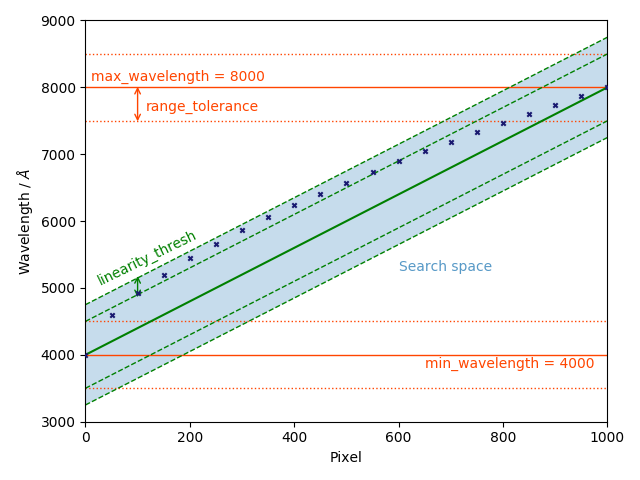
\includegraphics[width=\columnwidth]{plots/figure_1_threshold_plot.png}
    \caption{This illustrate how the \texttt{linearity\_thresh},
    \texttt{range\_tolerance} and the wavelength limits restrict the parameter
    space in the Hough space to significantly reduce the possible solution Hough
    pairs.}
    \label{fig:threshold}
\end{figure}

\subsubsection*{iii. \texttt{set\_ransac\_properties()}}
After supplying the atlas, we also need to define the properties of the RANSAC
operations. It needs the knowledge of both the atlas and the set of Hough pairs
so it cannot be predefined unless it is already deployed in some routine or
automated processing that the fitting parameters are already well known to
achieve desired output quality. The closely spaced Hough candidates can be
removed by setting \texttt{filter\_close} to \texttt{True}, where the peaks with
higher intensity among the closely spaced lines will be kept.

\subsubsection*{Step 2 -- Supply atlas}
An atlas can be loaded from the built-in list of cleaned NIST list with
\texttt{load\_atlas()}, the intensity of the lines are also included.
However, there is no easy way to account for the response function of
the detector without field-flattening and flux calibration, which in turn
requires wavelength calibration. The intensity setting should only be
used for removing faint lines. It is also possible to, and in fact
recommended, for users to provide a user-defined set of atlas with the
function \texttt{add\_user\_atlas()}. This can significantly improve
both the quality of fit as well as the speed of the fitting process.

\subsubsection*{Step 3 -- Configure the operations in Hough space}
The set of Hough pairs are generated with \texttt{set\_peaks()} which uses
\texttt{\_generate\_pairs()} to
\begin{enumerate}
    \item Pair up \texttt{peaks} (piexls) and \texttt{atlas} (wavelength)
    \item If \texttt{constrain\_poly} is set to \texttt{True},
        \texttt{Delaunay} from \texttt{scipy} is usd to remove outlying points.
    \item Order the pairs into a sorted list of [(peak 1, atlas 1),
        (peak 2, atlas 2), ..., (peak n, atlas n)]
    \item Optionally, append the known (peak, atlas) pairs with
        \texttt{set\_known\_pairs()} which are used as anchor(s) when solving
            for the solutions. This function has to be used with extreme
            caution, a set of wrong \textbf{known pairs} will guarantee
            poor or failed fit.
\end{enumerate}

\subsubsection*{Step 4 -- Run Hough Transform}
When executing the \texttt{\_do\_hough\_transform()}, the Hough parameters
will be propagated to the HoughTransform instance immediately before
executing the \texttt{generate\_hough\_points()} and
\texttt{bin\_hough\_points()} to generate the set of 
(1)~\texttt{hough\_points}, and (2)~\texttt{hough\_lines}. A HoughTransform
instance can be saved and loaded as \texttt{npy} or plain text \texttt{json}
files.

\subsubsection*{Step 5 -- Fit for the solution}
Most of the parameters were already set in with the three functions described
in step 1. At this point, only the fitting parameters are remained to be
configured: the number of iterations -- \texttt{max\_tries}, the degree of
polynomial to be fitted (\texttt{fit\_deg}), a starting set of polynomial
coefficients~(\texttt{fit\_coeff}), the acceptance threshold~
(\texttt{fit\_tolerance}) and the type of polynomial which can be chosen
from \texttt{ploy} for basic polynomial function, \texttt{legendre} or Legendre
polynomial function and \texttt{chebyshev} Chebyshev polynomial function. The
\texttt{brute\_force} can be set to True to discard the \texttt{max\_tries}
and try all possible combination in the given parameter space. The
\texttt{progress} is set to True by default to use the \texttt{tqdm} package
to show the progress of the fit.

The \texttt{fit()} function handles the heavy duty using the
\texttt{\_solve\_candidate\_ransac()}. It starts from getting the possible
wavelength solution of all the peaks for the given \texttt{hough\_line}, which
generates the \texttt{candidates} that contain the (1)~Hough solution wavelength,
(2)~atlas wavelength, and (3)~weight of the solution. The most common weighted
candidates will then be chosen with the \texttt{\_get\_most\_common\_candidates()}
by counting and returning the \texttt{top\_n} most common Hough solution wavelength.
The fit will stop and return nothing if the number of candidates is smaller than
the (degree of the polynomial + 1). From the Hough pairs, an interpolated 2D
density map is built in the Hough space, which is used as a weight map,
\texttt{weight}, in the fitting process. The pixel-wavelength solution will be
solved with the chosen polynomial function. The fit will be discarded if the two
lowest polynomials coefficients are outside the combined tolerance limits. The
absolute difference between the solutions and the atlas will give us the
uncertainties, \texttt{err}, of the solution. The \texttt{cost} function can
be computed by combining the \texttt{err} and \texttt{weight}. If the new cost
is lower, the new solution will be accepted.

An optional function \texttt{match\_peaks} is also available to refine the
fitted solution. It comes in two modes, the first is a more stable and
conservative way to refit the solution by searching for the wavelength-calibrated
peaks that are within the given tolerance limit from the atlas supplied. This
can give a marginally better fit, particularly reducing the root-mean-squared
measured. The second mode can be enabled by setting \texttt{refine} to
\texttt{True}, in this case, the small perturbation will be added to the accepted
set of polynomial coefficients and then a minimisation routine will be used to
fit for the new polynomial.

\subsubsection*{Other Utilities}
\texttt{RARCAL} comes with three built-in diagnostic plots, the most basic
one is the \texttt{plot\_arc} function which plot the arc spectrum
supplied along with the detected peaks. The other two are far more useful:
the \texttt{plot\_search\_space()} shows the search area in Hough space and
the final sets of Hough lines that were used in the solution; the
\texttt{plot\_fit()} displays the wavelength calibrated arc spectrum, the
residual of the solution as a function of wavelength, and the fitted polynomial
function as a function of wavelength.

\section{Test and Example Cases}

\subsection{Testing framework with simulated spectra}

One of the goals of \texttt{RASCAL} is to be agnostic to the choice of calibration
lamp or target. With  this in mind, it is not necessary to simulate a specific
lamp for testing. Since RASCAL also only requires peak locations, it is therefore not necessary to simulate flux noise, but it may be necessary to add jitter to peak locations.

A major challenge in assessing fitting performance is the requirement for ground truth. Metrics such as fitting error is not sufficient, as this does not eliminate the possibility that of a low-error but incorrect solution. We therefore use metrics such as repeatability and convergence.

\subsection{Worked Examples}

LT/SPRAT, GTC/OSIRIS, WHT/ISIS, INT/IDS, NTT/EFOSC, LCO/FLOYDS

\section{Stability}

In order to compare the quality of wavelength calibration, the repeatability and
convergence rates when using an automatic line list vs manual line list, we repeat the
wavelength calibration of an arc taken with the LT/SPRAT Xe lamp 1000 times at a
maximum number of trials at 25, 50, 100, 150, 200, 250, 500, 1000, 2000, and 5000.
Both the automatic and manual line lists are only referring to a set of wavelengths
of the template arc lines. The set of peaks used in both cases are identical, which
were determined automatically.

In figure~\ref{fig:coefficients}, we show the distributions of the five polynomial
coefficients in each of the cases for comparison. The better the repeatability, the
smaller the distribution is (a large kurtosis). It is clear that there is a correlation
between the size of the \texttt{max\_tries} and the kurtosis of the distributions. And
the manual line list is showing a more rapid convergence as it has a faster rate of
growth in the kurtosis, although, the two modes do not usually reach the same maximum
kurtosis as a manual line list is pruned to guarantee a unique set of solutions given a
sufficiently large \texttt{max\_tries} while the auto line lists may give the best fit
solutions coming from different local minima depending on the initial conditions of
the finite sampling.

The root-mean-squares of the residual from the $1000 \times 11$ fits are shown in the
violin plots in Fig.~\ref{fig:rms}. The quality of fit does not increase with the size
of \texttt{max\_tries}, but the distributions become smaller. This means the
repeatability is higher at larger \texttt{max\_tries}. This is not surprising, given
it is unreliable and in fact a bad practice to rely on a single quantity to determine
the quality of fit. In the auto line list mode, the spread as a function of
\texttt{max\_tries} is consistently larger than in manual mode due to multiple local
minima coming from fitting spurious lines.

\begin{figure}[h]
    \centering
    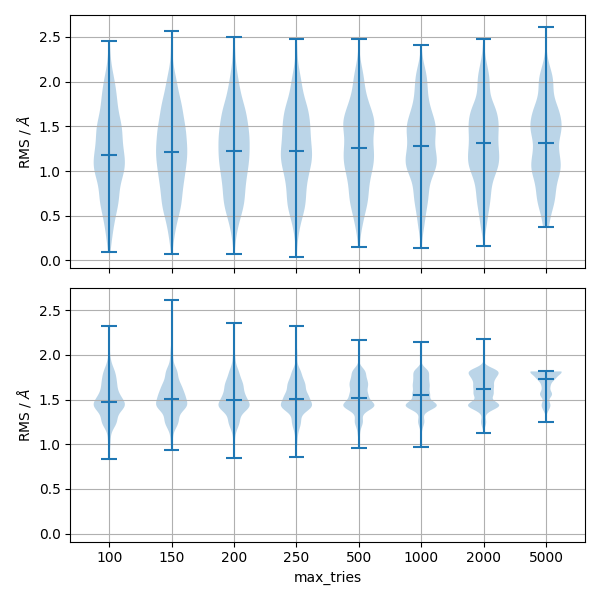
\includegraphics[width=\columnwidth]{plots/figure_2_rms.png}
    \caption{The distribution of the 1000 RMS values at the 8 \texttt{max\_tries} for
    auto line list (top) and manual line list (bottom). The convergence rate is much
    faster and the solution is much more stable when a known line list is provided.}
    \label{fig:rms}
\end{figure}


\begin{figure}[h]
    \centering
    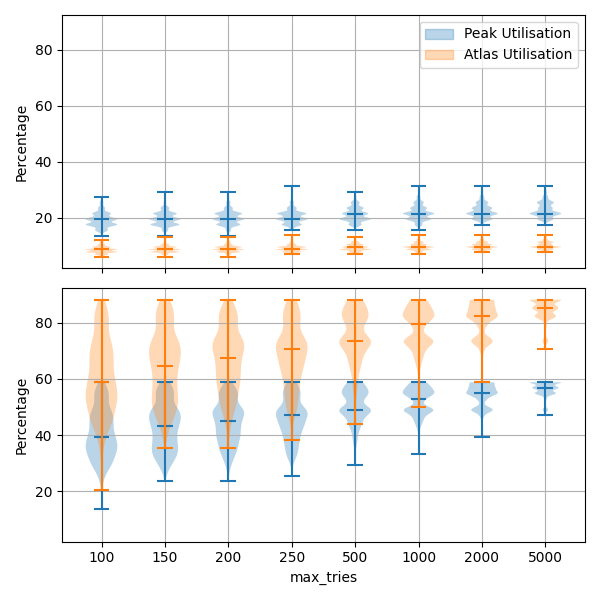
\includegraphics[width=\columnwidth]{plots/figure_3_peak_atlas_utilisation.png}
    \caption{The distribution of the 1000 \texttt{peak\_utilisation} and
    \texttt{atlas\_utilisation} percentage at 8 choices of \texttt{max\_tries} for auto
    line list (top) and manual line list (bottom). The low utilisation fraction in the
    top figure indicates that the auto line list contains much more lines than the
    number of peaks being detected, which makes it much more likely to fit for a wrong
    solution, as well as limiting the computing performance. The much higher
    utilisation fraction in the manual list demonstrates that \texttt{rascal} has a
    high repeatability despite the trial samples are drawn completely randomly in the
    first place.}
    \label{fig:peak_utilisation}
\end{figure}


\begin{figure*}[h]
    \centering
    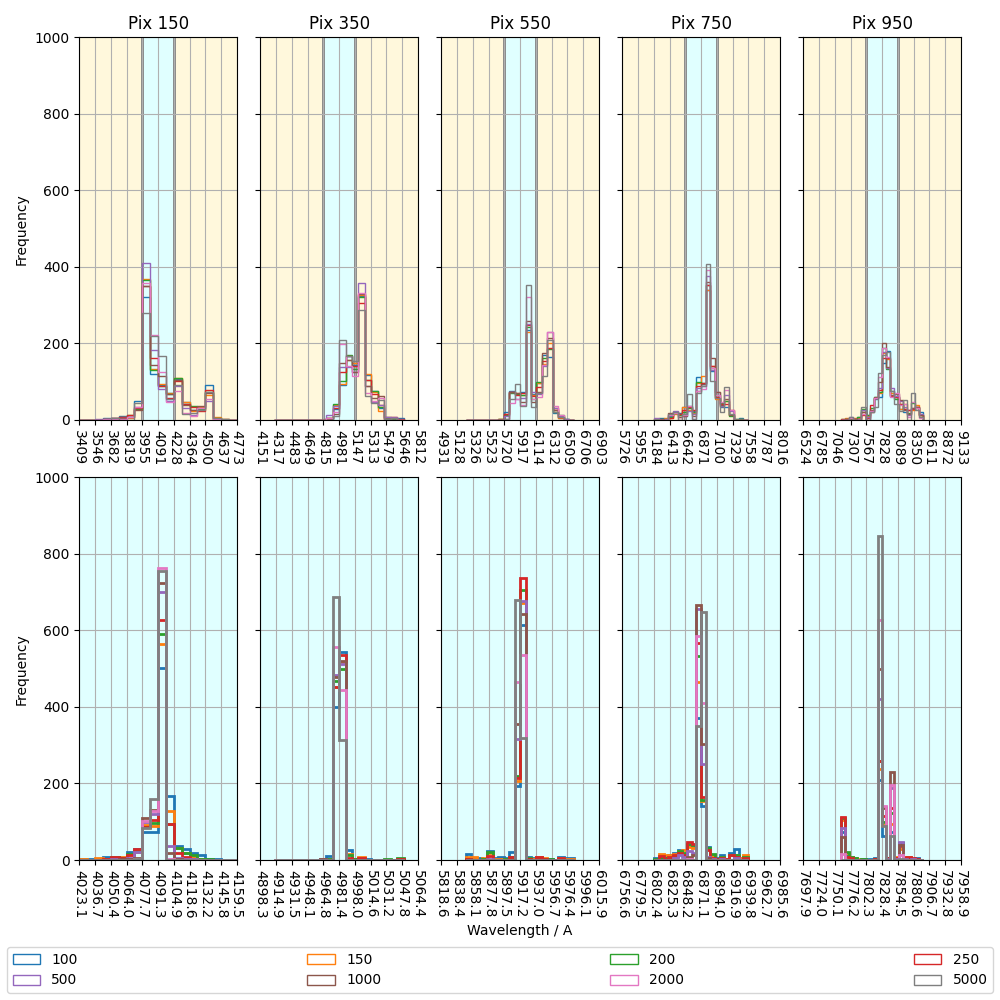
\includegraphics[width=\textwidth]{plots/figure_4_wavelengths.png}
    \caption{From left to right, they show the distributions of the wavelength
    solution at pixel 150, 350, 550, 750 and 950 at the 8 \texttt{max\_tries} with
    automatic line list (top), and manual line list (bottom). Pixel 150 and 950 are
    roughly at the two ends of the usable spectral wavelength range. The
    grid spacing in each sub-figure corresponds to $10\times$ and $1\times$ the
    resolution~($\Delta\lambda$) at that wavelength, respectively. The light blue
    shaded regions show the identical wavelength range in each column. There is a
    clear pattern of a narrower distribution with larger \texttt{max\_tries}. It
    is also clear that manual line list outperforms auto line list significantly.
    The statistics can be referred to Table~\ref{tab:stats}.}
    \label{fig:wavelengths}
\end{figure*}

The repeatability is illustrated in a different way in Fig.~\ref{fig:heatmap} by
plotting the heatmaps of the deviations from the true fit as a function of the pixels
across the detector. For perfect fitting every time, it should give a delta function
at $\Delta \lambda = 0$ at all pixels, which would appear as a bright horizontal line.
In the case of auto line lists, there are notably more deviated fits compared to
those using a manual line list. 

\begin{figure}[h]
    \centering
    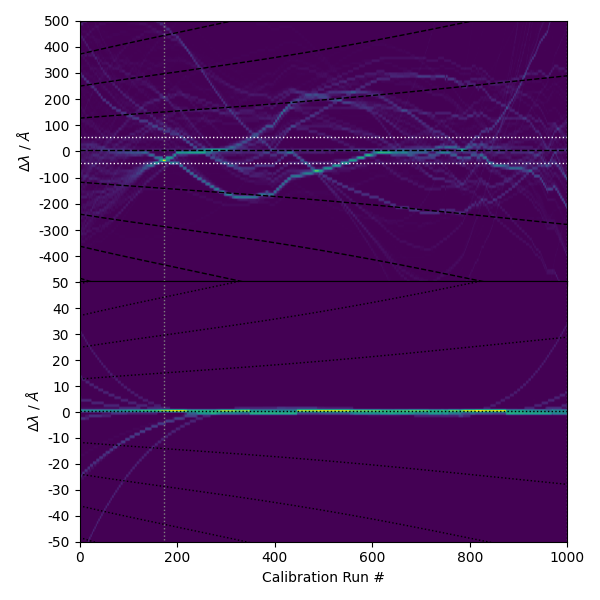
\includegraphics[width=\columnwidth]{plots/figure_5_heatmap.png}
    \caption{The heatmaps showing the deviation of the fitted wavelengths from the
    true value. The x-axis shows the calibration ID, where they are sorted by the
    fitted wavelength value at pixel 0. Note the difference in the scale in the y-axis.
    The use of auto line list (top) is giving good rough guesses most of the time,
    but it is clear that the manual line list completely outperforms the automatic
    one. The black dashed line in the top panel denotes 10 times the resolution that
    the spectrograph could resolve. The black dotted line in the bottom panel indicates
    the resolving power of spectrograph. The white dotted vertical lines denote the
    last usable peaks from the arc spectrum. The white dotted horizontal
    lines in the top panel mark the equivalent regions shown at the bottom. }
    \label{fig:heatmap}
\end{figure}

\begin{landscape}
\begin{table}
    \centering
    \begin{tabular}{|c|c|ccccc|c|ccccc|}
        \hline
        Grating & \texttt{max\_tries} & c0 & c1 & c2 & c3 & c4 & RMS & $\lambda_{150}$ & $\lambda_{350}$ & $\lambda_{550}$ & $\lambda_{750}$ & $\lambda_{950}$\\
        \hline
        \hline
          \multirow{16}{*}{\shortstack{LT/SPRAT\\(auto)}}
              & \multirow{2}{*}{100} & 3430.91  & 3.89110   & 8.11195e-3    & -1.77023e-5  & 1.10558e-8    & 1.20   & 4142.95  & 5193.43  & 6091.33  & 6942.16  & 8275.98\\
              &                      & (277.53) & (2.66040) & (1.341420e-2) & (2.50719e-5) & (1.55446e-8)  & (0.48) & (198.09) & (124.61) & (165.96) & (224.55) & (1087.80)\\\cline{2-13}
              & \multirow{2}{*}{150} & 3441.27  & 3.67420   & 8.73202e-3    & -1.80828e-5  & 1.09435e-8    & 1.21   & 4133.38  & 5185.83  & 6096.39  & 6942.60  & 8222.24\\
              &                      & (275.03) & (2.55439) & (1.259104e-2) & (2.35177e-5) & (1.44915e-8)  & (0.47) & (182.90) & (119.30) & (163.08) & (218.29) & (940.63)\\\cline{2-13}
              & \multirow{2}{*}{200} & 3431.77  & 3.86114   & 7.74110e-3    & -1.61698e-5  & 9.75522e-9    &  1.22  & 4135.48  & 5184.56  & 6099.49  & 6946.96  & 8168.27\\
              &                      & (270.60) & (2.53238) & (1.218320e-2) & (2.20195e-5) & (1.319168e-8) & (0.47) & (189.04) & (123.13) & (162.76) & (215.11) & (794.29)\\\cline{2-13}
              & \multirow{2}{*}{250} & 3426.09  & 3.82252   & 8.08717e-3    & -1.69782e-5  & 1.03540e-8    & 1.24   & 4129.37  & 5182.08  & 6097.55  & 6955.42  & 8232.91\\
              &                      & (271.56) & (2.48186) & (1.211745e-2) & (2.25815e-5) & (1.38574e-8)  & (0.46) & (185.86) & (124.23) & (159.47) & (207.24) & (845.67)\\\cline{2-13}
              & \multirow{2}{*}{500} & 3389.71  & 3.79888   & 8.64679e-3    & -1.77277e-5  & 1.05346e-8    & 1.26   & 4099.60  & 5176.56  & 6109.29  & 6957.06  & 8183.65\\
              &                      & (257.78) & (2.44981) & (1.196522e-2) & (2.27548e-5) & (1.41504e-8)  & (0.45) & (170.86) & (127.02) & (162.26) & (213.51) & (829.18)\\\cline{2-13}
              & \multirow{2}{*}{1000} & 3425.42  & 3.91589   & 7.44165e-3    & -1.53946e-5  & 9.17279e-9    & 1.28   & 4132.93  & 5185.19  & 6108.35  & 6956.00  & 8133.96\\
              &                       & (270.52) & (2.46457) & (1.176760e-2) & (2.15525e-5) & (1.288359e-8) & (0.45) & (180.70) & (126.75) & (160.07) & (194.94) & (627.35)\\\cline{2-13}
              & \multirow{2}{*}{2000} & 3397.81  & 3.85994   & 7.74098e-3    & -1.53905e-5  & 8.90982e-9    & 1.31   & 4103.55  & 5170.90  & 6117.14  & 6973.32  & 8112.66\\
              &                       & (249.37) & (2.26615) & (1.066695e-2) & (1.96646e-5) & (1.183229e-8) & (0.45) & (166.04) & (126.99) & (153.13) & (184.01) & (547.28)\\\cline{2-13}
              & \multirow{2}{*}{5000} & 3437.69  & 3.79338   & 7.43939e-3    & -1.50070e-5  & 8.89499e-9    & 1.30   & 4127.94  & 5166.75  & 6091.63  & 6950.74  & 8133.86\\
              &                       & (264.11) & (2.23694) & (1.060192e-2) & (2.00503e-5) & (1.228653e-8) & (0.46) & (173.75) & (126.16) & (150.86) & (203.43) & (604.73)\\\hline\hline
         \multirow{16}{*}{\shortstack{LT/SPRAT\\(manual)}}
              & \multirow{2}{*}{100} & 3515.46  & 3.46559   & 3.14713e-3   & -3.61417e-6  & 1.55256e-9   & 1.50   & 4094.70 & 4982.28 & 5914.30 & 6851.42 & 7813.93\\
              &                      & (105.64) & (1.03231) & (3.76259e-3) & (5.80846e-6) & (3.07476e-9) & (0.23) & (22.77) & (9.95)  & (26.44) & (82.38) & (198.66)\\\cline{2-13}
              & \multirow{2}{*}{150} & 3503.96  & 3.60646   & 2.58294e-3   & -2.72403e-6  & 1.08389e-9   & 1.52   & 4094.41 & 4982.11 & 5914.83 & 6855.46 & 7808.52\\
              &                      & (82.64)  & (0.81248) & (3.02430e-3) & (4.76675e-6) & (2.54765e-9) & (0.22) & (18.45) & (4.79)  & (21.71) & (59.78) & (158.04)\\\cline{2-13}
              & \multirow{2}{*}{200} & 3500.89  & 3.65013   & 2.40555e-3   & -2.44954e-6  & 9.57549e-10  & 1.52   & 4094.75 & 4982.46 & 5916.22 & 6861.19 & 7819.28\\
              &                      & (84.46)  & (0.80184) & (2.92103e-3) & (4.49597e-6) & (2.38484e-9) & (0.22) & (21.98) & (7.82)  & (16.93) & (51.86) & (132.35)\\\cline{2-13}
              & \multirow{2}{*}{250} & 3493.40  & 3.71641   & 2.163411e-3  & -2.07230e-6  & 7.64816e-10  & 1.51    & 4092.93 & 4981.79 & 5917.07 & 6865.37 & 7822.68\\
              &                      & (64.56)  & (0.60146) & (2.16526e-3) & (3.37330e-6) & (1.837343e-9) & (0.20) & (15.42) & (3.45)  & (10.55) & (40.75) & (120.48)\\\cline{2-13}
              & \multirow{2}{*}{500} & 3487.26  & 3.78006   & 1.92412e-3   & -1.70572e-6  & 5.77711e-10   & 1.53   & 4092.10 & 4981.53 & 5917.42 & 6867.81 & 7822.94\\
              &                      & (49.28)  & (0.41727) & (1.39933e-3) & (2.07474e-6) & (1.100292e-9) & (0.19) & (13.27) & (2.23)  & (4.61)  & (18.65) & (61.91)\\\cline{2-13}
              & \multirow{2}{*}{1000} & 3483.98 & 3.80699   & 1.84359e-3   & -1.61122e-6  & 5.48483e-10   & 1.55   & 4091.34 & 4981.41 & 5917.63 & 6870.04 & 7829.77\\
              &                       & (42.25) & (0.33934) & (1.04425e-3) & (1.42173e-6) & (7.12646e-10) & (0.17) & (11.07) & (1.12)  & (0.74)  & (4.51)  & (30.27)\\\cline{2-13}
              & \multirow{2}{*}{2000} & 3483.41 & 3.82264   & 1.76931e-3   & -1.49324e-6  & 4.89931e-10   & 1.60   & 4091.82 & 4981.40 & 5917.47 & 6870.68 & 7830.50\\
              &                       & (26.17) & (0.23186) & (7.3718e-4)  & (9.9813e-7)  & (4.87991e-10) & (0.17) & (5.00)  & (0.51)  & (0.66)  & (1.46)  & (15.20)\\\cline{2-13}
              & \multirow{2}{*}{5000} & 3478.03 & 3.87929   & 1.56648e-3   & -1.20105e-6  & 3.45073e-10   & 1.68   & 4091.29 & 4981.36 & 5917.25 & 6871.13 & 7828.41\\
              &                       & (20.82) & (0.17392) & (5.1839e-4)  & (6.5910e-7)  & (3.02712e-10) & (0.15) & (4.40)  & (0.50)  & (0.48)  & (0.49)  & (5.23)\\\hline
    \end{tabular}
    \caption{The median and 1 standard deviation values of the polynomial coefficients (c0 through c4), root-mean-squared (RMS) of the is fitted wavelength solution, and the five wavelength value at pixel 150 to 950 in 200 increment.}
    \label{tab:stats}
\end{table}
\end{landscape}

\section{Distribution}
The \textsc{RASCAL} is released under the BSD (3-Clause) License. The
source code is hosted on \textsc{Github}, which can be found at
\verb+https://github.com/jveitchmichaelis/rascal+, the tagged copied together
with the DOI of each version can be found at
\textsc{zenodo} \verb+https://zenodo.org/record/4117517#.YQfq2I4zYrQ+.
For simpler installation process, they are also available at Python
Package Index~(PyPI): \verb+https://pypi.org/project/rascal/+ such that
users can install the software by a simple command of 
\begin{verbatim}
    pip install rascal.
\end{verbatim}
While the development version can be installed with
\begin{verbatim}
pip install git+https://github.com/
    jveitchmichaelis/rascal@dev
\end{verbatim}

A rich resource of examples is available at
\verb+https://github.com/jveitchmichaelis/rascal-example+
where \verb+Jupyter+ notebooks are available to demonstrate the wavelength
calibration of the following long-slit instruments: (1)~NTT/EFOSC/Grism11,
(2)~Gemini GMOS longslit mode, (3)~GTC/OSIRIS/R1000B, (4)~KECK/DEIMOS/830G,
(5)~LT/SPRAT/Red, and (6)~WHT/ISIS/R300R. The examples cover elements
He, Ne, Ar, Cu, Kr, Xe, and Hg.

%--------------------------------------------------------------------
\section{Conclusions}

\textcolor{red}{More stuff here.}

Auto line list should be used to assist the preliminary line list selection
but not used at production level due to the relatively low repeatibility.
It can narrow down a subset of lines that can be adopted for full
automation with high reliability once quality check is performed by human.


\section*{Acknowledgements}
%%%%%%%%%%%%%%%%%%%%%%%%%%%%%%%%%%%%%%%%%%%%%%%%%%%%%%%%%%%%%%%%%%%%%%%%%%%%%%%%
MCL is supported by a European Research Council (ERC) grant under the European
Union’s Horizon 2020 research and innovation program (grant agreement number
833031).


%%%%%%%%%%%%%%%%%%%%%%%%%%%%%%%%%%%%%%%%%%%%%%%%%%%%%%%%%%%%%%%%%%%%%%%%%%%%%%%%
\section*{Data Availability}

%%%%%%%%%%%%%%%%%%%% REFERENCES %%%%%%%%%%%%%%%%%%

% The best way to enter references is to use BibTeX:

\bibliographystyle{rasti}
\bibliography{rascal} % if your bibtex file is called example.bib


%%%%%%%%%%%%%%%%%%%%%%%%%%%%%%%%%%%%%%%%%%%%%%%%%%

%%%%%%%%%%%%%%%%% APPENDICES %%%%%%%%%%%%%%%%%%%%%

%\appendix

%\section{Some extra material}

%%%%%%%%%%%%%%%%%%%%%%%%%%%%%%%%%%%%%%%%%%%%%%%%%%


% Don't change these lines
\bsp	% typesetting comment
\label{lastpage}
\end{document}

% End of rasti_template.tex

